% History
% 12/06/2024  (岸)	修論下書き用texファイル作成
% 12/12/2024  (岸)	フォントサイズを11pt, 行間を1.5に設定
% コンパイルの仕方
% 		uplatex chapter1_v1.tex
% 		upbibtex chapter1_v1
% 		uplatex chapter1_v1.tex
% 		uplatex chapter1_v1.tex
% 		dvipdfmx chapter1_v1.dvi

% フォントサイズを11ptに設定
\documentclass[a4paper,11pt,nomag]{jsreport}

\usepackage[dvipdfm,truedimen]{geometry}
\geometry{top=22mm,bottom=22mm,left=22mm,right=22mm}
%% jsclasses系で文字サイズ11pt や 12pt をクラスオプションに指定すると,
%% 長さが拡大されるため,nomagオプションを併用している.
%% https://oku.edu.mie-u.ac.jp/~okumura/jsclasses/ のFAQをよく読むこと.

%\usepackage{layout}
%\usepackage[utf8]{inputenc} %不要かも
\usepackage[T1]{fontenc} %utf8フォントエンコーディング指定
\usepackage{lmodern} % 11pt, nomag を使っているので
% CloudLaTeX の場合は下の1行を有効にすること
% \AtBeginDvi{\special{pdf:mapfile ptex-ipaex.map}}
\usepackage{array}
\newcommand{\bhline}[1]{\noalign{\hrule height #1}}  
\newcommand{\bvline}[1]{\vrule width #1}
\renewcommand{\baselinestretch}{1.5} % 教授が赤修正を入れやすいように行間を1.5に設定
\usepackage[subrefformat=parens]{subcaption}
\usepackage[dvipdfmx]{graphicx} % dvipdfmx を前提としている
\usepackage[dvipdfmx]{color}
\usepackage{caption}
\usepackage{subcaption}
\usepackage{bbm}
\usepackage{multirow}
\usepackage{arydshln}
\usepackage{here} % 図表の位置決め用
\usepackage{amsmath,amssymb}% 数式用
\usepackage{url}      % URL等記載用.\verbより便利
\usepackage{enumerate}
\usepackage{midpage}

% サブキャプションのフォーマットを調整
\renewcommand\thesubfigure{(\alph{subfigure})}
\captionsetup[subfigure]{labelformat=simple, labelsep=space}

\begin{document}
\setcounter{chapter}{2}

\chapter*{深層学習を用いた動物分類に関する既存研究}

\section{赤外線画像に対する既存研究}

気候変動や人口増加が生態系に与える影響を把握し,野生動物と人間の持続可能な共存を実現することは,重要な課題である.
この課題を解決するため,生態系モニタリングの重要性が世界的に高まっている\cite{zwerts2021, bandaru2024}.
生態系モニタリングの手法として,監視カメラなどを用いた観測が広く採用されており,特定地域における動物種の個体数推定だけでなく,環境に対する各動物種の生態観察や研究が行われている\cite{trolliet2014}.
中でも,カメラトラップは,観察者による直接的な介入を最小限に抑えることが可能であり,観察者の存在が個体の行動に与える影響を軽減することができるため,野生動物の監視ツールとして広く活用されている\cite{本郷2018, abood2023}.
カメラトラップは,赤外線センサなどを用いた自動撮影により人的労力を削減することができ,近年のデジタルカメラの高性能化に伴い長期間にわたる連続的なモニタリングが可能である.
一方で,カメラトラップを使用した生態系モニタリングでは複数箇所にカメラトラップを設置するため,膨大な画像枚数を取得することも多く \cite{kays2020, si2014},記録された画像・動画中から人手による動物の有無や種の推定は多大なアノテーションコストを要する\cite{thangaraj2023}.
加えて,種の分類には専門的な知識が必要であることも作業員確保によるコスト面での課題である.
さらに,技術革新は今後も進むと予想されるのに対して,アノテーションコストを著しく下げることは困難であるため,このギャップは今後一層拡大していくと予想される\cite{安藤2019}.
したがって,これらの課題を解決するため,カメラトラップによって撮影された画像・動画中から自動で動物を検出・識別する手法の実現が望まれている.

近年では,画像処理技術と機械学習を用いた野生動物の自動識別手法が研究されている.
2012年の画像処理タスクに関連する深層学習技術の登場以降,画像処理分野の様々な分野においてCNNに基づく手法が盛んに研究されている.
また,その多くの分野においてCNNは高い性能を実現しており,カメラトラップによる動物識別に関する研究においてもCNNを用いた手法がいくつか提案されている.
Tanら \cite{tan2022}は,2014年から2020年にかけて撮影された約25,000枚の自作データセットを用いて,YOLOv5,FCOS(Fully Convolutional One-Stage Object Detection),Cascade R-CNNの3つの検出ネットワークでの比較検証,および映像に適用した動物認識の性能を評価している.
Tabakら \cite{tabak2019}は,全米5箇所で撮影された約300万枚のカメラトラップ画像を用いて,独自のCNNにより動物の画像分類を行っている.

しかしながら,上記のような既存研究の分類モデルを学習するために用いられた大規模なデータセットは,多くの撮影場所や数年間に及ぶ長期間の撮影によって蓄積された画像で構成されている.
したがって,これらの既存研究は,個人的な利用での撮影や狭い範囲の地域での撮影など,十分な画像データを収集できない状況には適していないため、実用面での課題が残る.
また,夜間に行動する動物の撮影には赤外線カメラを用いることが有効であるが,赤外線カメラで撮影された画像は色情報を含まないなど,可視光カメラで撮影された画像とは映り方が異なる.
したがって,真に実用的な夜間の動物モニタリングの実現に向けて,赤外線カメラを用いて撮影された少数の画像のみでも学習可能な深層学習モデルについての検討が急務である.

このような既存研究の課題解決に向けた研究として,少数の赤外線画像を用いた動物分類が挙げられる.
Kishiら \cite{kishimoto2023}は,米国南西部の140箇所で撮影された画像3,000枚を用いて,CNNによる少数の赤外線画像を用いた動物分類を行っている.
先行研究では,少数データを用いた効率的な深層学習モデルの学習を目的とするFSLの分野において有効な手法である転移学習とデータ拡張の赤外線画像に対する有効性が検証された.
転移学習は,事前に大量のデータを用いて学習したモデルを新しいタスクに適用する手法であり,先行研究では,画像認識タスクで一般的に用いられるImageNetデータセットとImageNetデータセットを擬似赤外線化した画像,さらに数式から生成されたフラクタル画像による転移学習の有効性が検証された.
一方,データ拡張については,一般的な画像変換に加え,画像の一部をマスクし隠すことでモデルの汎化性能を向上させるRandom Erasingや,複数の画像処理を組み合わせることで新しい画像を生成しモデルの頑健性を向上させるAugmixなどの有効性が検証された.
実験の結果,転移学習では疑似赤外線画像,フラクタル画像,ImageNetの順に効果が高いことが示され,データ拡張については,最新の手法であるAugMixが特に有効であることが明らかになった.

Kishiらの研究では,新規地域に対する深層学習モデルの適用開始時を想定しており,学習に使用する画像は1クラスあたり50枚としているが,実運用を想定すると1クラスあたり50枚程度の画像収集すら困難な場合も考えられる.
また,評価実験における評価用データセットでは学習用データセットと同じ動物種のみが使用されており,モデルの適用地域に生息する全ての動物種がモデルに登録されている閉集合が仮定されている.
モデルの実運用開始時において,対象地域に生息する全ての動物種のデータを網羅的に収集することは現実的ではない.
従来の分類モデルでは,学習データに含まれないモデルに未登録の動物を正しく識別できず,登録済みのクラスに強制的に分類されてしまうオープンセット問題が存在する.
% 特に重要な課題として,モデルの学習に使用されるデータに含まれる動物種が少ない場合,実用時には学習データに含まれなかった動物が出現することが挙げられる.
% 一般的な分類モデルは,そういった未見の動物を正しく識別できず,学習済みのクラスに強制的に分類してしまう.
図 \ref{fig:non_osr}は,従来の分類モデルが未登録の動物を識別できない例を示している.

\begin{figure}[tbp]
  \centering
  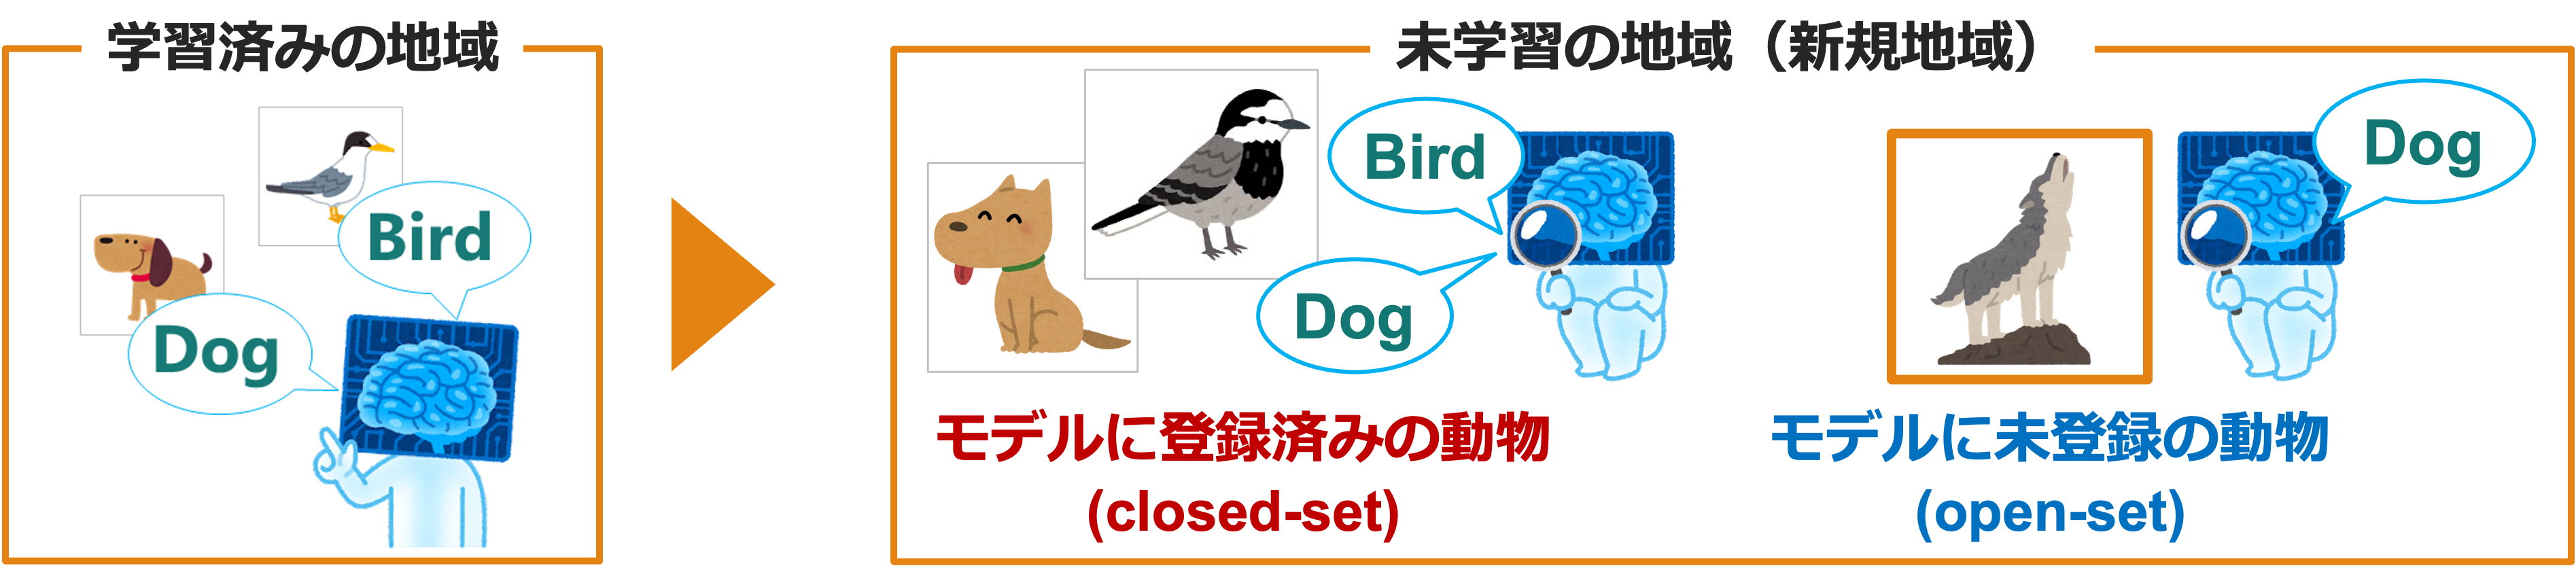
\includegraphics[width=\linewidth, keepaspectratio]{image/non_osr.png}
  \caption{従来の分類モデルによるオープンセット問題の例}
  \label{fig:non_osr}
\end{figure}

図\ref{fig:non_osr} に示される通り,犬と鳥のみを学習したモデルを新規地域に適用した場合,モデルに登録済みの犬や鳥は分類できるが,未登録の動物であるオオカミは登録済みの動物種に強制的に分類されてしまう.
このような誤分類はモデルの精度低下へと繋がるため,未登録の動物種を適切に検出できるOSRモデルの開発が急務となっている.

以降,モデルに登録されているクラスセットをクローズドセット(closed-set),モデルに未登録のクラスセットをオープンセット(open-set)と呼ぶ.


\subsection{Few-Shot Open-Set Recognitionに関する既存研究}

昨今の第3次人工知能 (Artificial Intelligent, AI) ブームにおける機械学習システムの高い性能や実用的な成果は,主にクローズドセットタスクにおいて達成されてきた.
これらのシステムでは,学習用データセットと評価用データセットに同一のクラスが含まれることを前提としており,システムの評価は学習時に登録されたオブジェクトクラスのみを対象として実施される.
しかしながら,より実用的なシステムの実現を目指す場合,現実的な問題設定として「オープンセット問題」への対応が不可欠である\cite{geng2021survey}.
機械学習ベースのシステムの利用が進むにつれ,幅広いアプリケーションにおいて高い頑健性を備えた手法が要求されており,OSR技術に注目が集まっている\cite{sun2023survey}.
OSRは,学習時に想定していないクラスのデータが入力された場合でも,システムを頑健に機能させるためのアプローチの1つとして位置付けられている.
図 \ref{fig:osr}にOSRにおける未登録データの検出プロセスの一例を示す.
\begin{figure}[tbp]
  \centering
  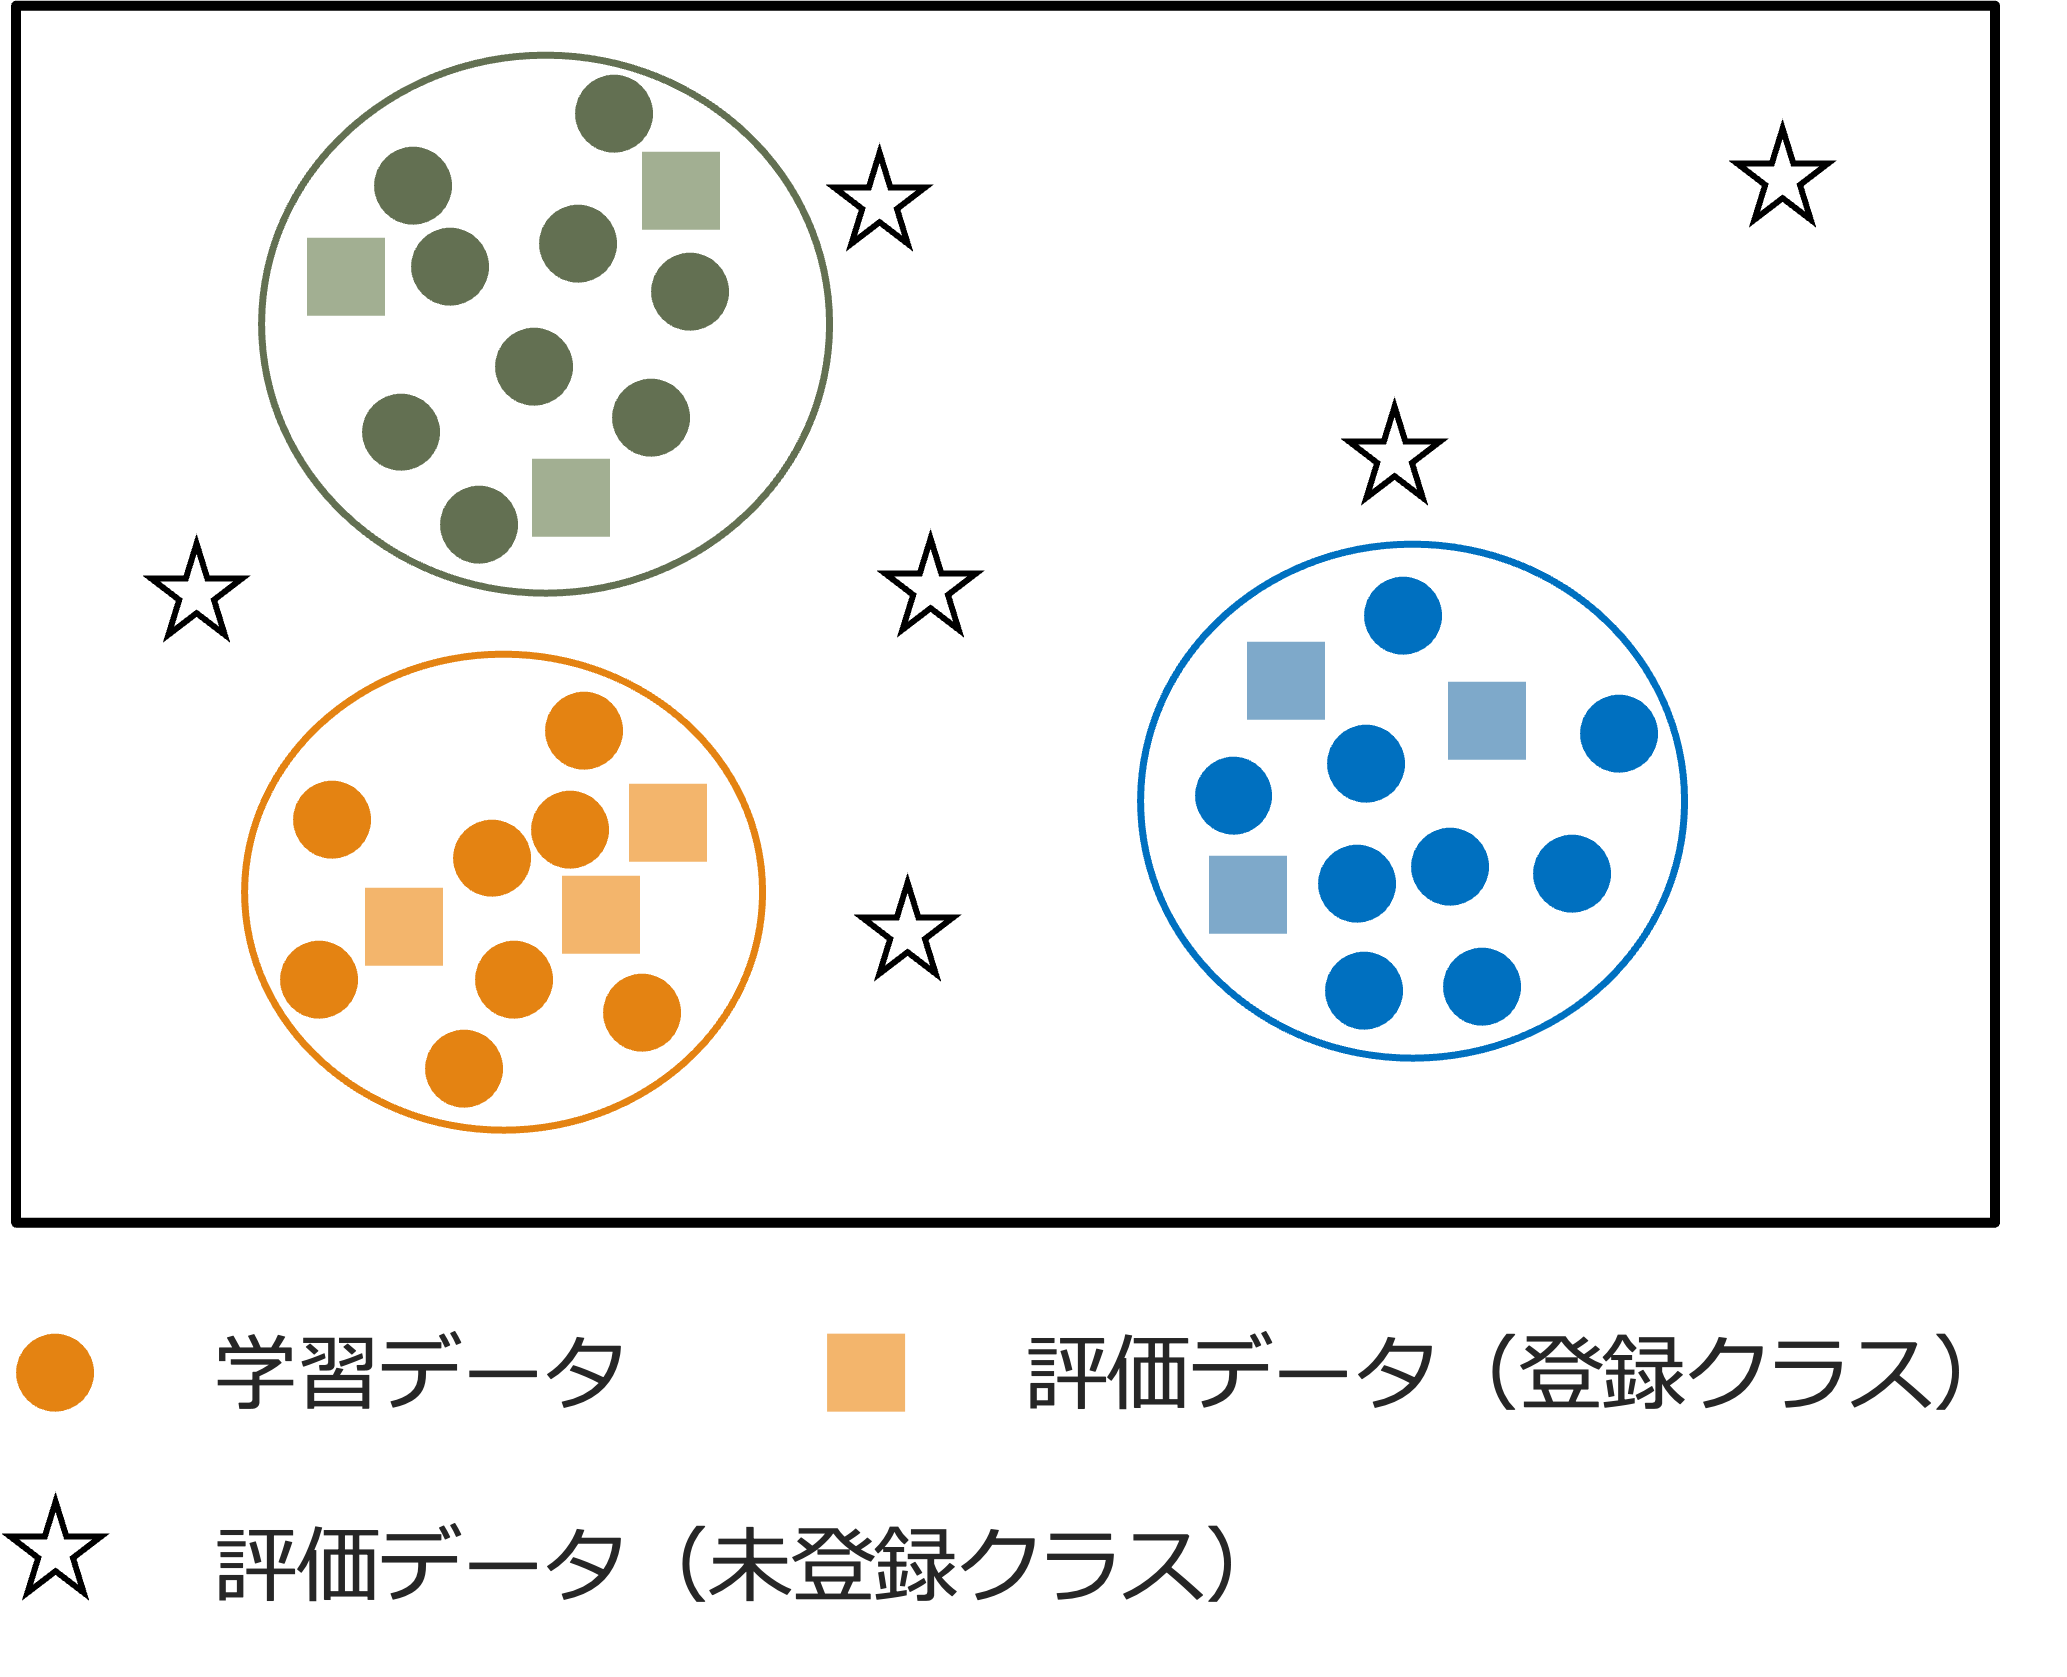
\includegraphics[width=0.6\linewidth, keepaspectratio]{image/osr.png}
  \caption{OSRにおける未登録データの検出プロセスの一例}
  \label{fig:osr}
\end{figure}
既存の分類モデルでは未登録データを既存クラスに分類してしまう課題があったが,分類対象の画像の特徴量と既存クラスの類似度が特定の閾値を下回る場合に未登録クラスとして検出することで,この課題を解決することが可能となった.

未登録クラスを考慮しない場合,システムの不適切な開発につながり,その有用性が著しく制限されることとなる.
しかし,実世界の動的な環境における認識・分類タスクに適した正確かつ完全なモデルの構築には多くの課題が存在する\cite{mahdavi2021survey}.
これは,学習時に想定していないクラスが無数に存在する可能性があり,それらすべてを事前に予測して学習データに含めることが現実的ではないためである.
% とくに,深層学習モデルはデータ駆動型のモデルであり,学習データと評価データが同一の確率分布に従うという仮定に大きく依存している.
% そのため,未登録クラスのデータが入力された場合でも,登録クラスの1つとして高い信頼度で誤分類してしまう問題が指摘されている\cite{sun2023survey}.
とくに,深層学習モデルはデータ駆動型のアプローチのため,適切な帰納バイアスを獲得するために大量の学習データを必要とする.
同様に,既存のOSR手法においても大量の学習データの利用を前提としており,その適用範囲は局所的な場面に限定されている.

% そこで,Liu\cite{peeler}らは,学習用データセットのサイズに依存しないオープンセット認識の実現を目指し,新たな認識フレームワークであるFew-Shot Open-Set Recognition (FSOSR) を提案した.
% 具体的には,大規模な学習データが利用可能な環境とわずかな学習データしか利用できない学習環境という,2つの極端な状況のいずれにおいても有効に機能する汎用的な手法を検討した.
% 既存のOSRの問題設定では,大量の学習データを用いてタスクを解くのに対し,FSLの問題設定では学習データが非常に少ないという違いにより,既存のOSR 手法がFSL への適用が困難であることが挙げられる.

この課題に対し,近年ではFew-Shot Open-Set Recognition(FSOSR)という新たな研究分野が注目を集めている.
FSOSRは,少数の画像データからの効率的な学習による正確な分類を行うことと,学習データに存在しないデータを未登録クラスとして検出・拒絶できるモデルの構築を目的とした分野である\cite{peeler}.
% FSOSRでは,従来のFSL手法とOSR手法を単純に組み合わせただけでは,登録クラスの分類と未登録クラスの検出の双方を高い精度で実現することは困難であることが示されている\cite{peeler}.
% 少数のデータを用いた分類 (FSL) と未登録データの識別 (OSR) を両立することは極めて困難な課題である.

Jeongら \cite{snatcher}は,変換一貫性(transformation consistency)という概念に基づき,未登録クラスを検出するSnaTCHerを提案した.
これは,類似した入力データは特徴量空間での変換後も近い位置関係を保つという性質を利用している.
% 具体的には,クエリ特徴量とその予測クラスのプロトタイプを入れ替えた後,特徴量変換を適用し,変換前後の差異を測定する.
未登録クラスの入力データは,登録クラスとは異なる特徴空間を形成する傾向があるため,変換後の特徴量は既知クラスのプロトタイプから大きく離れることが期待される.
プロトタイプとは,登録クラスを代表する特徴ベクトルのことであり,登録クラスから得られた特徴量の平均値を取ることによって生成される.
この手法の最大の利点は,疑似的な未知クラスサンプルを必要としない点である.
OSRなどにおける従来手法が未登録クラスの分布を直接推定しようとしていたのに対し,SnaTCHerは特徴量の相対的な変換問題として扱うことで,より効率的な学習を実現した.
また,様々な特徴量変換手法との組み合わせ実験により,分類性能を低下させることなく,未知クラスサンプルの検出性能を向上させることが確認された.

一方で,Huangら \cite{tane}は,閾値の設定に依存しない新しい手法としてTask-Adaptive Negative Envision (TANE)を提案した.
TANEは,登録クラスのプロトタイプから負例のプロトタイプを生成し,これを用いてタスクに応じた動的な拒否境界を学習する.
具体的に,登録クラスの代表点に注意機構を適用して負例のプロトタイプを生成し,入力データとの類似度が計算される.
もしすべての登録クラスに対する予測スコアが負例プロトタイプに対するスコアよりも低い場合,その入力データは未登録クラスとして拒否される.

本研究では,限られたデータに対する赤外線動物分類の実現に向けて新しい問題設定を提案するとともに,今後の赤外線動物分類タスクの発展のため様々な手法の有効性を検証する.

% 上記の問題の解決策として,メタ学習をFSOSR に応用した手法\cite{peeler} が提案された.
% メタ学習とは,FSL の分野において有効な手法の一種であり「学習方法を学習する」という概念に基づいた手法である.
% FSL に用いられるメタ学習では,モデルは少数のデータを用いた分類に適応する必要があるため,少数データの分類を適切に行うことができる特徴抽出を学習する.
% 本研究では,いくつかあるメタ学習手法の中でもPrototypical Networks(ProtoNet)\cite{protonet} を用いたメタ学習に着目する.
% ProtoNet は,一般的な深層学習モデルが画像をヘッドを用いてクラス分類確率まで畳み込み分類を行うのに対して,畳み込みを行う直前の特徴ベクトルを利用することにより画像の分類を行う手法である.
% クラス分類確率と特徴ベクトルの関係について,一般的な深層学習モデル構造の例としてViT のモデル構造を図2.2.2に示す.
% 一般的な分類問題では,クラス分類確率が最も高いクラスに画像が分類されるが,FSL においては,少量のデータを使用するため画像の特徴が豊富に表現されている特徴ベクトル同士を比較することにより効果的に分類を行うことが可能となる.

% FSL の問題設定では,いくつかの見本となるデータが渡された際,分類を行いたい対象データが見本データのどのクラスに属するかを正確に分類することが求められる.
% この時,正確な分類を行うためには,分類モデルは対象画像から特徴を抽出する際に,見本データに類似する特徴ベクトルを抽出できる必要がある.
% メタ学習では,追加データを用いて,対象データと見本データの特徴ベクトル間の類似度を高めるような特徴抽出を繰り返し学習することで,新しいデータに対しても正確な分類ができるようにモデルの訓練を行う.

% FSOSR に拡張されたメタ学習においては,未見データを識別するために,未見データを他の見本クラスとは類似度が低くなるような損失を追加することで,未見の識別と分類の両方を学習することを可能とした.

% 本研究では,2.1 章で述べた少数の赤外線画像における動物分類の問題解決のために新しい問題設定を提案するとともに,提案する問題設定におけるメタ学習の有効性について検証を行う.


% ここから参考文献bibtexの設定
\bibliographystyle{../kishiIEEEtr}
\bibliography{../references}

\end{document}